\section{Infix Proofs}
The security of the original NIPoPoWs protocol suffers under velvet fork conditions for the case of
infix proofs as well. Again, since blocks containing incorrect interlink pointers are accepted in the 
chain, the adversary may create an infix proof for a transaction included in a block mined on a
different chain. This attack is presented in detail in the following.

An infix proof attack when applying the original protocol under a velvet fork should be obvious
after our previous discussion. So consider the updated protocol for secure suffix proofs as
described in the previous section. A problem here is that in the updated protocol some blocks
are excluded from the interlink, while we should still be able to provide proofs for transactions
included in any block of the chain.

For this reason, let us naively consider an additional protocol patch suggesting to include
a second interlink data structure in each block, which will be updated without any block exclusion,
just as described in the original protocol and will be used for constructing infix proofs only. In
order to be secure we could think of allowing using pointers of the second interlink only for the
\textit{followDown} part of the algorithm. But still, the adversary may use an invalid pointer of a
block visited during the \textit{followDown} procedure and jump to a block of another chain providing 
a transaction inclusion proof concerning that block. This attack is illustrated in
Figure \ref{fig:infix_attack}.

\begin{figure}[h!]
	\begin{center}
		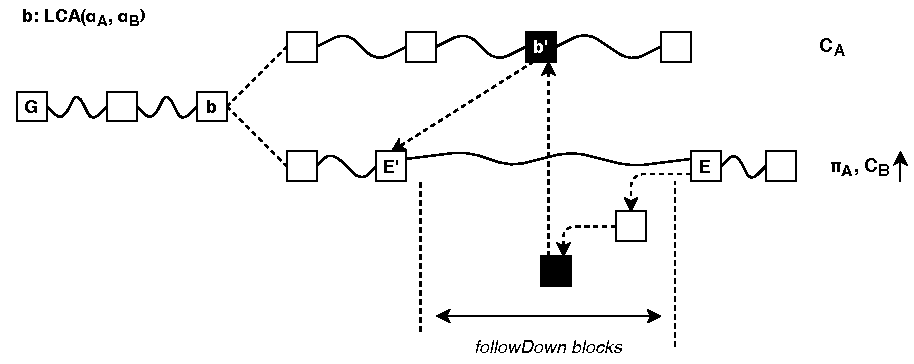
\includegraphics[width=0.9\columnwidth]{figures/infix_attack.pdf}
	\end{center}
	\caption{Adversarial fork chain $C_A$ and an adversarial infix proof based on the chain
	 adopted by an honest player. Wavy lines imply one or more blocks. Blocks generated by the
	 adversary are colored black. Dashed arrows represent interlink pointers included in the proof
	 as part of the \textit{followDown} procedure. The adversary provides infix proof for a
	 transaction in block b'. }
	\label{fig:infix_attack}
\end{figure}

Thus giving the ability to utilize invalid pointers even in a narrow block window can break the
security of our protocol. 

\subsubsection*{Protocol patch for NIPoPoWs infix proofs under velvet fork}
In order to construct secure infix proofs under velvet fork conditions, we suggest the following additional protocol patch: each upgraded miner constructs and updates an authenticated data structure for all the blocks in the chain. We suggest Merkle Mountain Ranges \emph{(MMR)} for this structure. Now a velvet block's header additionally includes the root of this MMR.

After this additional protocol change the notion of a smooth block changes as well. Smooth blocks are now considered the blocks that contain truthful interlinks and valid MMR root too. A valid MMR root denotes the MMR that contains all the blocks in the chain of an honest full node. Note that a valid MMR contains all the blocks of the longest valid chain, meaning both smooth and thorny. An invalid MMR constructed by the adversary may contain a block of a fork chain. Consequently an upgraded prover has to maintain a local copy of this MMR locally, in order to construct correct proofs. This is crucial for the security of infix proofs, since keeping the notion of a smooth block as before would allow an adversary to produce a block $b$ in an honest party's chain, with $b$ containing a smooth interlink but invalid MMR, so she could succeed in providing an infix proof about a block of a fork chain.

\subsubsection*{The velvet infix prover and verifier}
Considering this addtional patch we can now define the final algorithms for the honest miner, infix and suffix prover, as well as for the infix verifier. Because of the new notion of smooth block, the function \textit{isSmoothBlock()} of Algorithm \ref{alg:smooth_chain_suffix} needs to be updated, so that the validity of the included MMR root is also checked. The updated function is given in Algorithm \ref{alg:isSmoothBlock_infix}. Considering that input $\chain_S$ is computed using Algorithm \ref{alg:smooth_chain_suffix} with the updated \textit{isSmoothBlock'()} function, \emph{Velvet updateInterlink} and \emph{Velvet Suffix Prover} algorithms remain the same as described in Algorithms \ref{alg:update_interlink}, \ref{alg:velvet_suffix_prover} repsectively. The velvet infix prover  given in Algorithms \ref{alg:velvet_infix_prover}, \ref{alg:velvet_infix_verifier} respectively.
In order to keep the algorithm generic enough for any infix-sensitive predicate, we provide the steps needed until the verification of the block of interest and consider that the specific predicate can be answered by a known algorithm given the block of interest. 
Given that the verifier is already synchronized to the longest valid chain, the infix verification algorithm only has to confirm
the Merkle-Tree inclusion proof $\pi_{b'}$ for the block of interest $b'$.

Details about the construction and verification of an MMR and the respective inclusion proofs can be found in \cite{ct}.
Note that equivalent solution could be formed by using any authenticated data structure that provides inclusion proofs of size logarithmic to the length of the chain. We suggest MMRs because of they come with efficient update operations.

\begin{algorithm}[h]
	\caption{\label{alg:isSmoothBlock_infix}Function isSmoothBlock'() for infix proof support}
	\begin{algorithmic}[1]
			\Function{\sf isSmoothBlock'}{$B$}
				\If{$B = \mathcal{G}$}
					\State\Return{$\true$}
				\EndIf
				\For{$p \in B.\textsf{interlink}$}
						\If{$\lnot \textsf{isSmoothPointer}(B, p)$}
							\State\Return{$\false$}
						\EndIf
				\EndFor
				\State\Return{$\textsf{containsValidMMR}(B)$}
			\EndFunction
	\end{algorithmic}
\end{algorithm}

\begin{algorithm}[h]
	\caption{\label{alg:velvet_infix_prover}Velvet Infix Prover}
	\begin{algorithmic}[1]
			\Function{\sf ProveInfixVelvet}{$\chain_S, b$}
				\Let{(\pi,\chi)}{\textsf{ProveVelvet}(\chain_S)}
				\Let{\textsf{tip}}{\pi[-1]}
				\Let{\pi_b}{\textsf{MMRinclusionProof}(tip, b)}
				\State\Return{$(\pi_b,(\pi, \chi))$}
			\EndFunction
	\end{algorithmic}
\end{algorithm}

\begin{algorithm}[h]
	\caption{\label{alg:velvet_infix_verifier}Velvet Infix Verifier}
	\begin{algorithmic}[1]
			\Function{\sf VerifyInfixVelvet}{$b, (\pi_b,(\pi,\chi))$}
				\Let{\textsf{tip}}{\pi[-1]}
				\State\Return{\textsf{VerifyInclProof(tip.$root_{MMR}$, $\pi_b$, $b$)}}
			\EndFunction
	\end{algorithmic}
\end{algorithm}

%\subimport{./}{infix_maximum_delay.tex}
